


\documentclass[crop, tikz]{standalone}
\usepackage{tikz}
\usepackage{amssymb}
\usetikzlibrary{calc}
\usepackage{colortbl}

 
% Definition of circles
\def\firstcircle{(0,0) circle (1.5cm)}
\def\secondcircle{(0:2cm) circle (1.5cm)}
\def\innercircle{(-0.3,0) circle (0.8cm)}

\colorlet{circle edge}{black!80}
\colorlet{circle area}{gray!50}

\tikzset{filled/.style={fill=circle area, draw=circle edge, thick},
    outline/.style={draw=circle edge, very thick}}

\setlength{\parskip}{5mm}
 
 \begin{document}



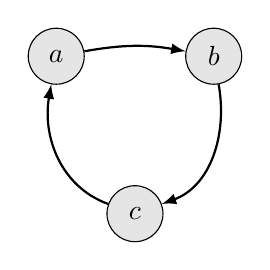
\begin{tikzpicture}
	
	\node[draw=black,fill=gray!20,circle,minimum width=0.28in] (a)  at (0,2) {$a$};
	\node[draw=black,fill=gray!20,circle,minimum width=0.28in] (b) at (2,2) {$b$};
	\node[draw=black,fill=gray!20,circle,minimum width=0.28in] (c) at (1,0) {$c$};
 
	\path[->,>=latex, draw=black,thick ] (a) to[looseness=1,in=170,out=10] (b);
	\path[->,>=latex,draw=black,   thick] (b) to[looseness=1,in=20,out=280] (c);
	\path[->,>=latex,draw=black,   thick] (c) to[looseness=1,in=260,out=160] (a);

\end{tikzpicture}
	
 
\end{document}


